\documentclass[10pt]{beamer}

\usepackage[utf8]{inputenc}
\usepackage{tcolorbox}
\usepackage{tikz}
\usepackage{tikz-3dplot}
\usetikzlibrary{intersections,calc,,angles,quotes,through}
\usepackage{amsmath}
\usepackage{graphicx}
\usepackage{cases}
\def \heart {\textcolor{blue}{$\heartsuit$} }
\def \C {\mathcal{C}}
\def \orthog {\underline{\perp}}
\def\arcos{\operatorname{arcos}}
\def\cos{\operatorname{cos}}
\def \deg {^{\circ}}

\newcommand{\vect}[1] {
  \overrightarrow{#1}}
  
\tcbset{%
	basic/.style={colframe=black,
		      colback=white,
		      top= 0mm,
		      bottom = 2mm,
		      boxsep=0mm
		      }
}
\tikzset{
    invisible/.style={opacity=0},
    visible on/.style={alt={#1{}{invisible}}},
    alt/.code args={<#1>#2#3}{%
      \alt<#1>{\pgfkeysalso{#2}}{\pgfkeysalso{#3}} % \pgfkeysalso doesn't change the path
    },
  }

    
\begin{document}  
    \beamertemplatenavigationsymbolsempty
    \setlength{\abovedisplayskip}{0pt}
    \setlength{\belowdisplayskip}{0pt}
    \frame{
	  
	  \frametitle{Q3 Septembre 2004.}
	  %\renewcommand{\theenumi}{\alph{enumi})}
	  On considère un triangle $ABC$ (non isocèle) du plan. On construit sur le côté
	  $BC$ et dans le plan du triangle $ABC$ deux triangles équilatéraux $BDC$ et $BD'C$.
	  Démontrer la relation \\ \medskip
	  $|\vect{AD}|^2 + |\vect{AD'}|^2 = |\vect{AB}|^2 + |\vect{AC}|^2 + |\vect{BC}|^2$.

	  \vfill
	  
	  \pause
	  % hypothèses et thèse
	  \begin{tcolorbox}[basic] 
	      \begin{columns}[t]
		 
		 \column{.52\textwidth}\centering
		      
		      \underline{Hypothèses} 
		      \begin{itemize}
		      \item $\Delta BDC, \Delta BD'C$ équilatéraux.
		      \end{itemize}

		  
		  \column{.5\textwidth}\centering
		      
		      \underline{Thèse} \\
		      \smallskip
		      $|\vect{AD}|^2 + |\vect{AD'}|^2$ \\ \smallskip$= |\vect{AB}|^2 + |\vect{AC}|^2 + |\vect{BC}|^2$.
		
	      \end{columns}
	  \end{tcolorbox}
    }

    \frame{ 
	  % résolution ex1
	  \begin{columns}[t]
		\column{.5\textwidth}\centering 
		

			\underline{Dessin}\\
			
				  \begin{figure}[h]
				  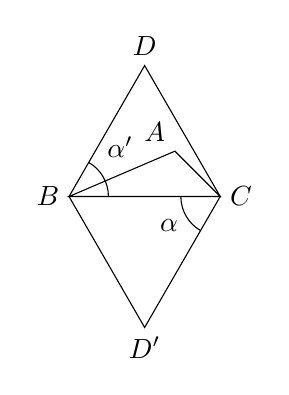
\begin{tikzpicture}[scale=0.48]
			          %projection ($(X)!(B')!(B)$)
			          %nommer chemin 'name path
			          %intersection \path [name intersections={of=d and gb,by=G}];
			          %animation  \draw[visible on=<1>] 
				  %           \draw[visible on=<{2,4}>]
				  %angle arc[radius = 6mm, start angle= 180, end angle= 225] node [below left,pos=0.3]{$\alpha$}
				  %angle \pic [draw,"$\alpha$", angle eccentricity=1.5] {angle = A'--A--B};
				  %perpendiculaire ($(A')!3cm!-90:(A)$)
				  
				  %TRIANGLE ABC
				  \coordinate[label= above left:$A$](A) at (0.8,1.2);
				  \coordinate[label=left:$B$](B) at (-2,0);
				  \coordinate[label=right:$C$](C) at (2,0);
				  \draw (A) -- (B) -- (C) -- cycle;
				  
				  %D
				  \draw (B) -- +(60:4) coordinate[label=above:$D$](D) -- (C);
				  %D'
				  \draw (B) -- +(-60:4) coordinate[label=below:$D'$](D') -- (C);
				  
				  %ANGLES
				  \pic [draw,"$\alpha '$", angle eccentricity=1.5,above] {angle = C--B--D};
				  \pic [draw,"$\alpha$", angle eccentricity=1.5] {angle = B--C--D'};
				  \end{tikzpicture}
				  \end{figure}
			
				  \begin{tcolorbox}[basic] 
				      
				    \smallskip
				    \underline{Hypothèses} 
				    \begin{enumerate}
				    \item $\Delta BDC, \Delta BD'C$ équilatéraux. 
				    \end{enumerate}
							      
				    \underline{Thèse} \\
				    \smallskip
				    $|\vect{AD}|^2 + |\vect{AD'}|^2$ \\ \smallskip$= |\vect{AB}|^2 + |\vect{AC}|^2 + |\vect{BC}|^2$.
				    \end{tcolorbox}
		
		
		\column{.5\textwidth}\centering
		
		\underline{Résolution}\\ \flushleft
		
		\begin{enumerate}
		 \item $\begin{cases}\alpha = \alpha ' = 60\deg \rightarrow BD \parallel CD', \\ 
		       |BD|=|CD'|.
		       \end{cases}$
		       
		\end{enumerate}	\medskip
		
		$\rightarrow \vect{BD}=\vect{D'C}$. \\ \medskip
		
		\begin{align*}
		 \vect{AD}=& \vect{AB} + \vect{BD}, \\
		 \vect{AD'}=& \vect{AC} + \vect{CD'}. \\[0.5em]		 
		\end{align*}
		\vspace{-5mm}
		\begin{align*}
		 &|\vect{AD}|^2 + |\vect{AD'}|^2 \\[0.3em]
		 &= |\vect{AB}|^2 + |\vect{AC}|^2 + 2|\vect{BD}|^2  \\
		          &\phantom{{}=1}+ 2\vect{BD}\cdot(\vect{CA} + \vect{AB}), \\[0.3em]
		 &= |\vect{AB}|^2 + |\vect{AC}|^2 +2\vect{BD}\cdot (\vect{CB} + \vect{BD}), \\[0.3em]
		 &= |\vect{AB}|^2 + |\vect{AC}|^2 +2\vect{BD}\cdot\vect{CD},
		\end{align*}

	   \end{columns}
   
    }
	
	\frame{ 
	  % résolution ex1
	  \begin{columns}[t]
		\column{.5\textwidth}\centering 
		

			\underline{Dessin}\\
			
				  \begin{figure}[h]
				  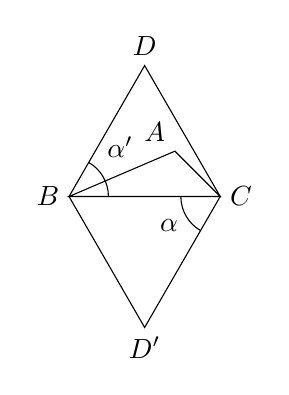
\begin{tikzpicture}[scale=0.48]
			          %projection ($(X)!(B')!(B)$)
			          %nommer chemin 'name path
			          %intersection \path [name intersections={of=d and gb,by=G}];
			          %animation  \draw[visible on=<1>] 
				  %           \draw[visible on=<{2,4}>]
				  %angle arc[radius = 6mm, start angle= 180, end angle= 225] node [below left,pos=0.3]{$\alpha$}
				  %angle \pic [draw,"$\alpha$", angle eccentricity=1.5] {angle = A'--A--B};
				  %perpendiculaire ($(A')!3cm!-90:(A)$)
				  
				  %TRIANGLE ABC
				  \coordinate[label= above left:$A$](A) at (0.8,1.2);
				  \coordinate[label=left:$B$](B) at (-2,0);
				  \coordinate[label=right:$C$](C) at (2,0);
				  \draw (A) -- (B) -- (C) -- cycle;
				  
				  %D
				  \draw (B) -- +(60:4) coordinate[label=above:$D$](D) -- (C);
				  %D'
				  \draw (B) -- +(-60:4) coordinate[label=below:$D'$](D') -- (C);
				  
				  %ANGLES
				  \pic [draw,"$\alpha '$", angle eccentricity=1.5,above] {angle = C--B--D};
				  \pic [draw,"$\alpha$", angle eccentricity=1.5] {angle = B--C--D'};
				  \end{tikzpicture}
				  \end{figure}
			
				  \begin{tcolorbox}[basic] 
				      
				    \smallskip
				    \underline{Hypothèses} 
				    \begin{enumerate}
				    \item $\Delta BDC, \Delta BD'C$ équilatéraux. 
				    \end{enumerate}
							      
				    \underline{Thèse} \\
				    \smallskip
				    $|\vect{AD}|^2 + |\vect{AD'}|^2$ \\ \smallskip$= |\vect{AB}|^2 + |\vect{AC}|^2 + |\vect{BC}|^2$.
				    \end{tcolorbox}
		
		
		\column{.5\textwidth}\flushleft
		
		$=|\vect{AB}|^2 + |\vect{AC}|^2 +2\vect{BD}\cdot\vect{CD}$, \\ \medskip
		$=|\vect{AB}|^2 + |\vect{AC}|^2 +2\vect{DB}\cdot\vect{DC}$, \\ \bigskip
		
		\heart $\vect{XY}\cdot\vect{XZ}=|\vect{XY}||\vect{XZ}|\cos(\widehat{ZXY})$. \\ \bigskip
		
		\begin{align*}
		\vect{DB}\cdot\vect{DC}=&|\vect{BD}||\vect{CD}|\cos(\widehat{BDC}), \\
				       =&\frac{|\vect{BC}|^2}{2}.
		\end{align*} \bigskip
		
		$=|\vect{AB}|^2 + |\vect{AC}|^2 + |\vect{BC}|^2$. \hfill $\qed$
		

	   \end{columns}
   
    }
  
\end{document}
